%!TEX root = main.tex

\section{Numerical solutions}
\label{sec:numerics}
\subsection{Identification of equilibrium branches}

We now switch to the study of  the nonlinear\comment[id=ALB]{Let's clarify our use of linear/nonlinear} regime  and we will resort to numerical calculations  to explore the system's behavior beyond the linear approximation.

In order to find the equilibrium branches we make use of a pseudo-arclength continuation technique implemented in the software AUTO~\cite{Doedel1981-sa}. It solves the nonlinear equations \ref{auto1} and \ref{auto2} in the case of rigid and compliant foundation, respectively, with the relative end displacement $\bar\epsilon$ treated as a continuation parameter. To discretize the boundary-value problem, it uses collocation with Lagrange polynomials, and in our simulations we had $N=300$ mesh points with $N_c = 5$ collocation nodes and activated mesh adaptation. 
\begin{figure}
% 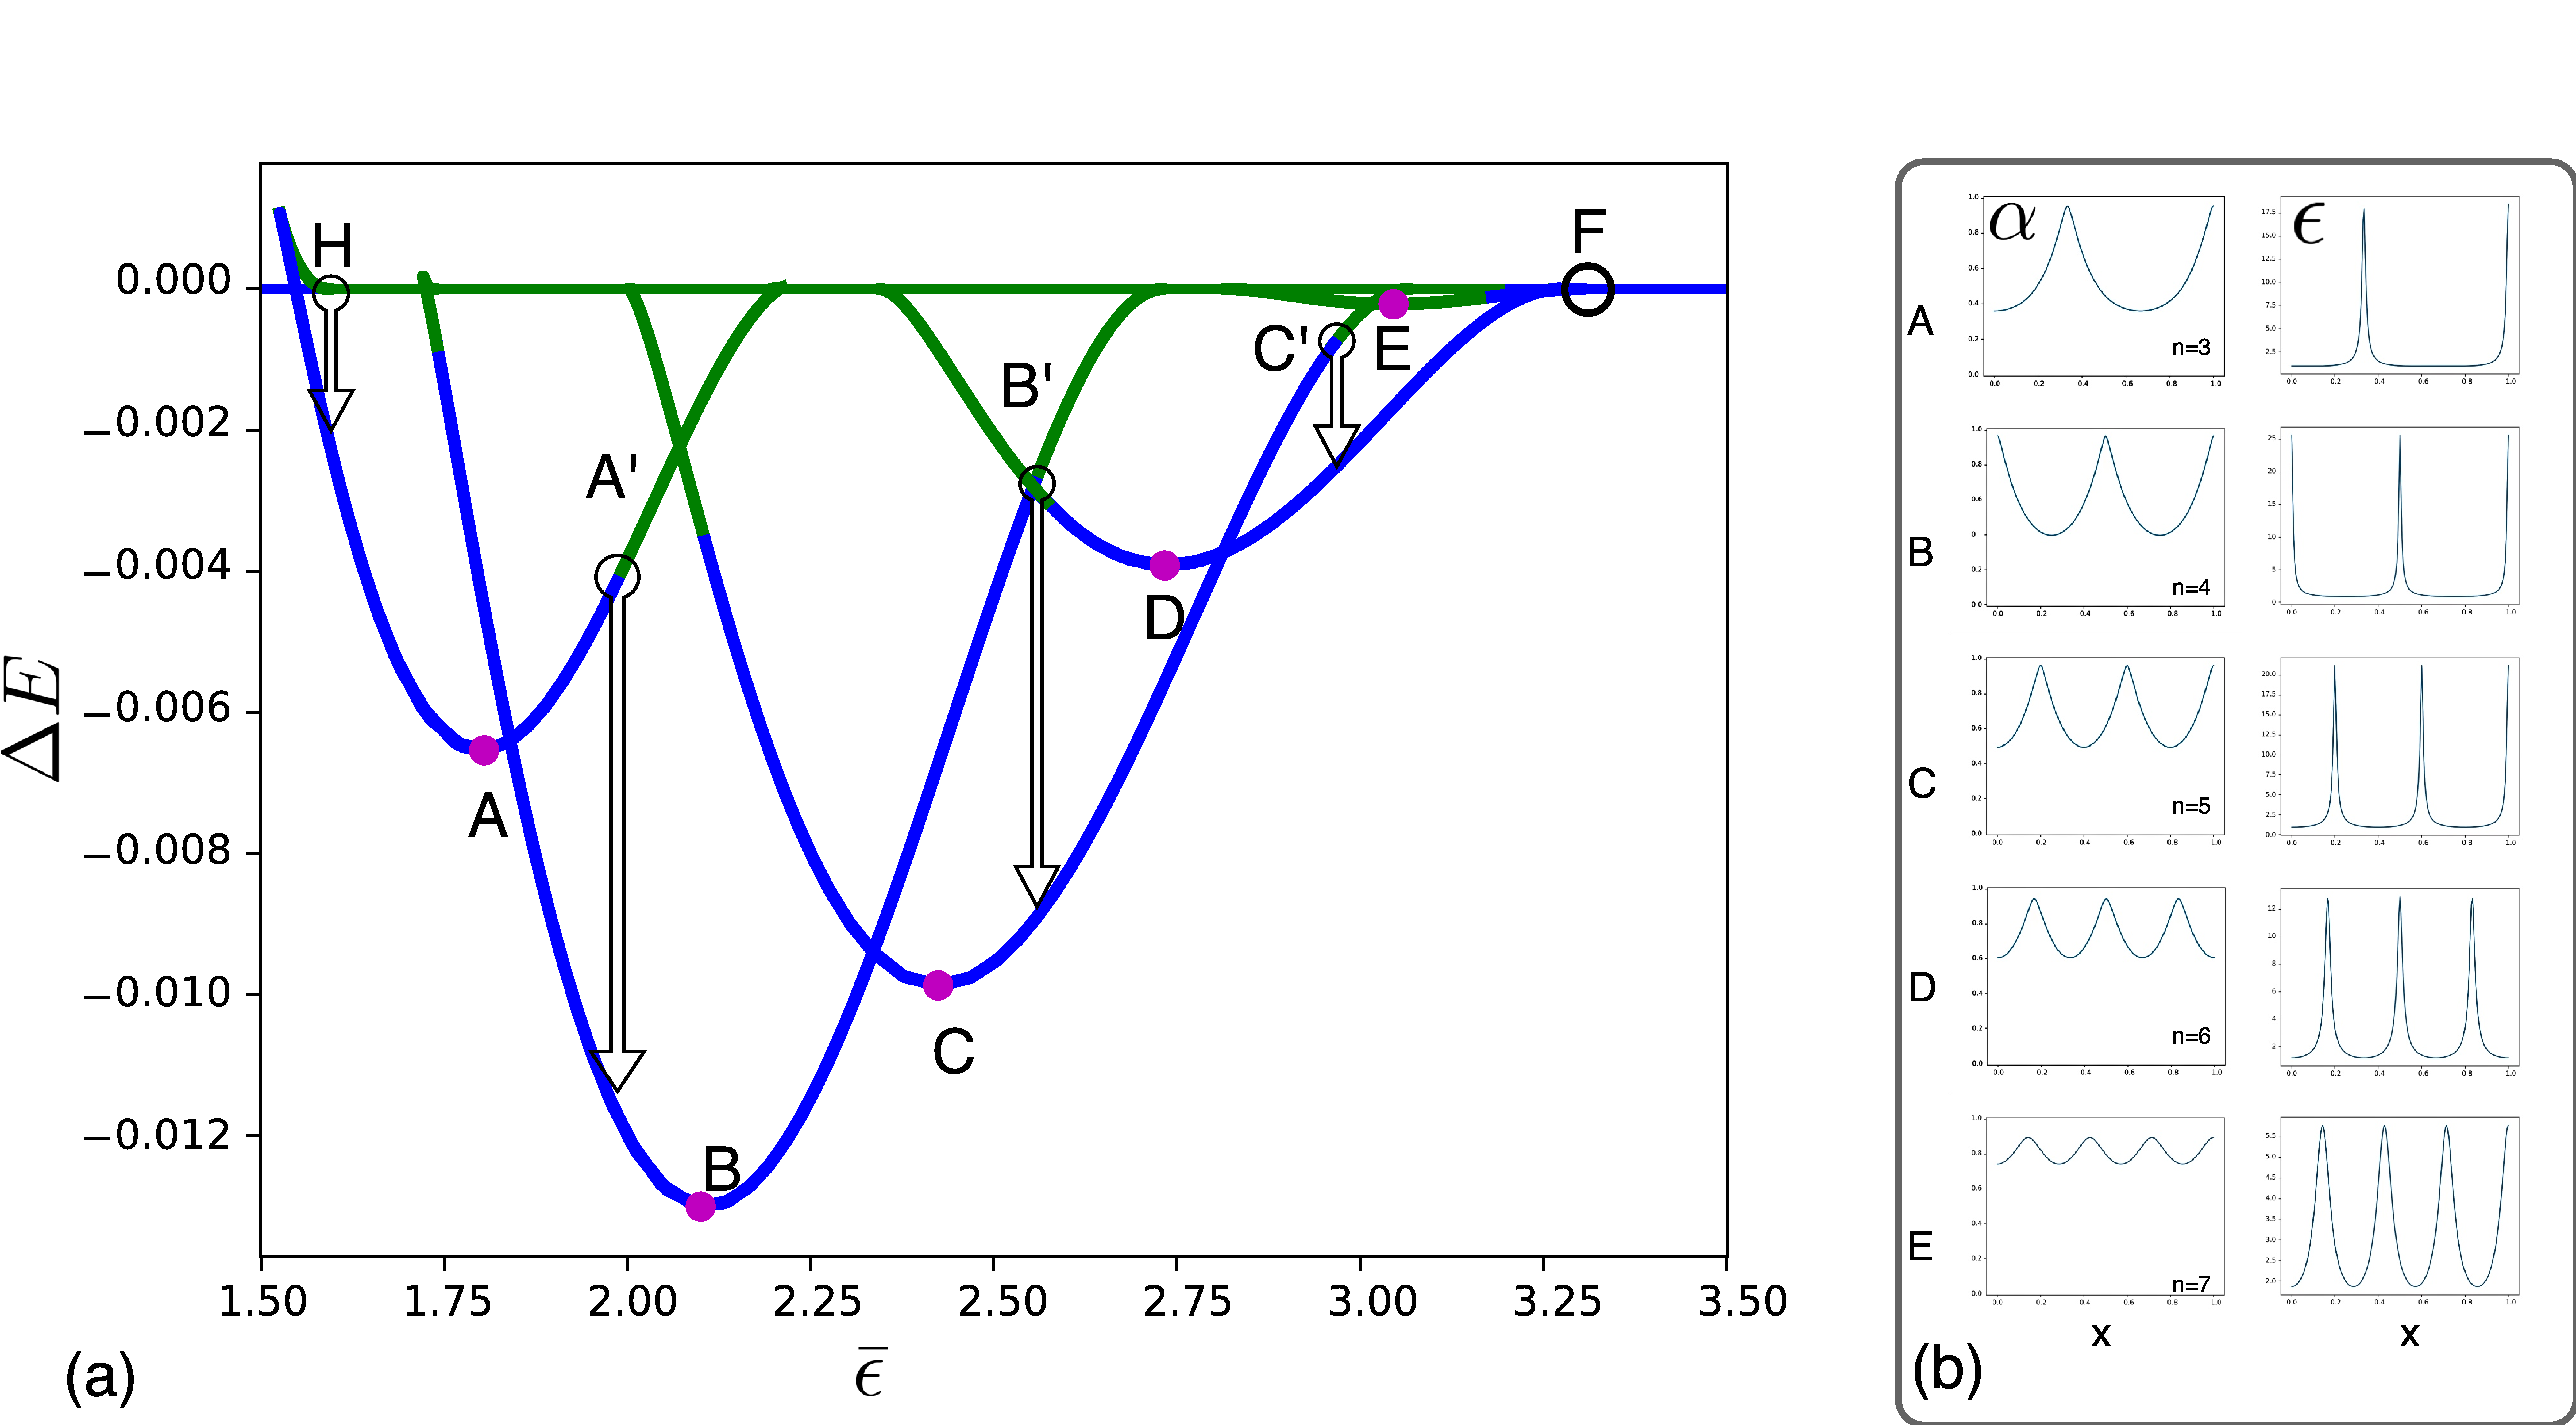
\includegraphics[scale=0.1]{./final_images/fig2.pdf}
\includegraphics[width=.8\textwidth]{../images/model_stiff_energy.pdf}
\includegraphics[width=.7\textwidth]{../images/model_stiff_fields.pdf}
    \caption{
% \todo[inline]{Add marker for $\ep_c$ in a), }
Equilibrium branches in the phase-field model of an elastic bar on rigid elastic foundation: (a) the energy difference $\Delta E$ between the affine and non-affine configurations. Stability of solutions is indicated by colors: blue denotes stability, while green indicates instability   via the numerical evaluation of the smallest eigenvalue of the stiffness matrix $\stiffmat$. Arrows indicate the anticipated branch switching events associated with the loss of stability; (b) the damage and strain profiles of the minimum energy configurations on each branch.}
    \label{fig:branches-stiff}
\end{figure}
In order to asses the stability of equilibrium branches, we use  the numerical evaluation of the smallest eigenvalue of the second variation by discretizing the integrals \eqref{hessian22} and   \eqref{hessian222} to construct the stiffness matrix
$\stiffmat$ and investigating numerically the sign of the minimal eigenvalue $\kappa$ of the corresponding discrete quadratic form \cite{Sanderson2016-ht}.  The finite element discretization of the displacement and damage field $(u, \alpha )$     with \( n_u \) displacement degrees-of-freedom 
$
\mathbf{u} = \{ u_1, \ldots, u_{n_u} \}^T 
$
and \( n_\alpha \) damage degrees-of-freedom 
$
\boldsymbol{\alpha} = \{ \alpha_1, \ldots, \alpha_{n_\alpha} \}^T
$ is given by 
$
u(\mathbf{x}) \approx u_{\text{FE}} (\mathbf{x}) := \sum_{i=1}^{n_u} \mathcal{N}^{(u)}_i(\mathbf{x}) u_i $
and $\alpha(\mathbf{x}) \approx \alpha_{\text{FE}} (\mathbf{x}) := \sum_{i=1}^{n_\alpha} \mathcal{N}^{(\alpha)}_i (\mathbf{x}) \alpha_i 
$
where $\mathcal{N}^{(u)}(\mathbf{x}) $ and $\mathcal{N}^{(\alpha)}(\mathbf{x}) $ are the finite element basis functions and  $u_h$ and  $\alpha_h$ are nodal values for the displacement and damage fields, respectively. We used quadratic one-dimensional finite elements with 3 nodes  whose   shape functions   ${\mathcal N}_i(x)$ at a node $i$  are given by ${\mathcal N}_1(\xi)=-0.5\xi(1-\xi)$, ${\mathcal N}_2(\xi)=-0.5\xi(1+\xi)$ and ${\mathcal N}_3(\xi)=-(1-\xi)(1+\xi)$, where $\xi$ is the isoparameteric coordinate. The discrete solution $u(x_i)$ provided at discrete nodes $x_i$ by AUTO was first interpolated using B-spline basis functions of degree 3 \cite{Grimstad2016-cq}, and then utilized to calculate the integrals \eqref{hessian22} and   \ref{hessian222} employing a three-point Gauss integration scheme. The fixed boundary conditions were enforced by removing the rows and columns corresponding to $x = 0$ and $x = 1$ from the stiffness matrices 
% $\mathbf{K}^i, i = 1, 2$
$\stiffmat$ and $\widetilde\stiffmat$. The explicit form of the stiffness matrix for the stiff substrate model is given by
\begin{equation}
    \stiffmat = 
    % \stiffmat^1=
    \begin{bmatrix}
\int_0^1[ \frac{1}{\lambda_2^2}{\mathcal N}_i{\mathcal N}_j + (1-\alpha)^2{\mathcal N}'_i{\mathcal N}'_j
%+\frac{1}{\lambda_2^2}{\mathcal N}_i {\mathcal N}_j
] dx&
-2\int_0^1(1-\alpha)u' {\mathcal N}'_i {\mathcal N}_j  dx\\
-2\int_0^1(1-\alpha)u' {\mathcal N}_i {\mathcal N}'_j dx
& \int_0^1 [ (2+u'^2){\mathcal N}_i{\mathcal N}_j +\lambda_1^2{\mathcal N}'_i{\mathcal N}'_j] dx
\end{bmatrix},
\label{eq:stifness1}
\end{equation}
and in the compliant substrate model it reads

\begin{equation}
    \stiffmatcompl=
    % /\stiffmat^2=
    \begin{bmatrix}
    \int_0^1[ \frac{1}{\lambda_2^2}{\mathcal N}_i{\mathcal N}_j + (1-\alpha)^2{\mathcal N}'_i{\mathcal N}'_j] dx&
-2\int_0^1(1-\alpha)u' {\mathcal N}'_i {\mathcal N}_j  dx&
-\int_0^1[\frac{1}{\lambda_2^2}{\mathcal N}_i {\mathcal N}_j]  dx\\

-2\int_0^1(1-\alpha)u' {\mathcal N}_i {\mathcal N}'_j dx&
 \int_0^1 [ (2+u'^2){\mathcal N}_i{\mathcal N}_j +\lambda_1^2{\mathcal N}'_i{\mathcal N}'_j] dx&
 0\\

-\int_0^1[\frac{1}{\lambda_2^2}{\mathcal N}_i{\mathcal N}_j ] dx
&0
&\int_0^1\frac{1}{\lambda_2^2}{\mathcal N}_i {\mathcal N}_j+r_s{\mathcal N}'_i {\mathcal N}'_j  dx
\end{bmatrix}.
\label{eq:stifness2}
\end{equation}
Our objective is to establish a branch switching strategy as part of our model's DEFINITION\comment[id=ALB]{Unclear}. This extension must ensure the system's re-stabilization following an instability in a dissipative manner. In a quasi-static scenario, it should involve the selection of a new locally stable equilibrium branch with inherently lower energy.  Considering applications in structural mechanics, our approach to selecting the new equilibrium branch involves utilizing a criterion of local energy minimization (LEM)\comment[id=ALB]{Acronyms, imho, make it harder to read by requiring extra mental buffer.}  which emulates the zero viscosity limit of overdamped viscous dynamics. This approach SETS ASIDE A global energy minimizing (GEM) strategy, which may be relevant in biomechanical applications~\cite{Salman2021-mn}. According to LEM protocol, during quasi-static loading, the system will remain in a metastable state (a local minimum of energy) until it becomes unstable. Subsequently, during an isolated switching event, the new equilibrium branch will be chosen using a descent algorithm \cite{Puglisi2005-lg}.
\begin{figure}
    %\centering
% 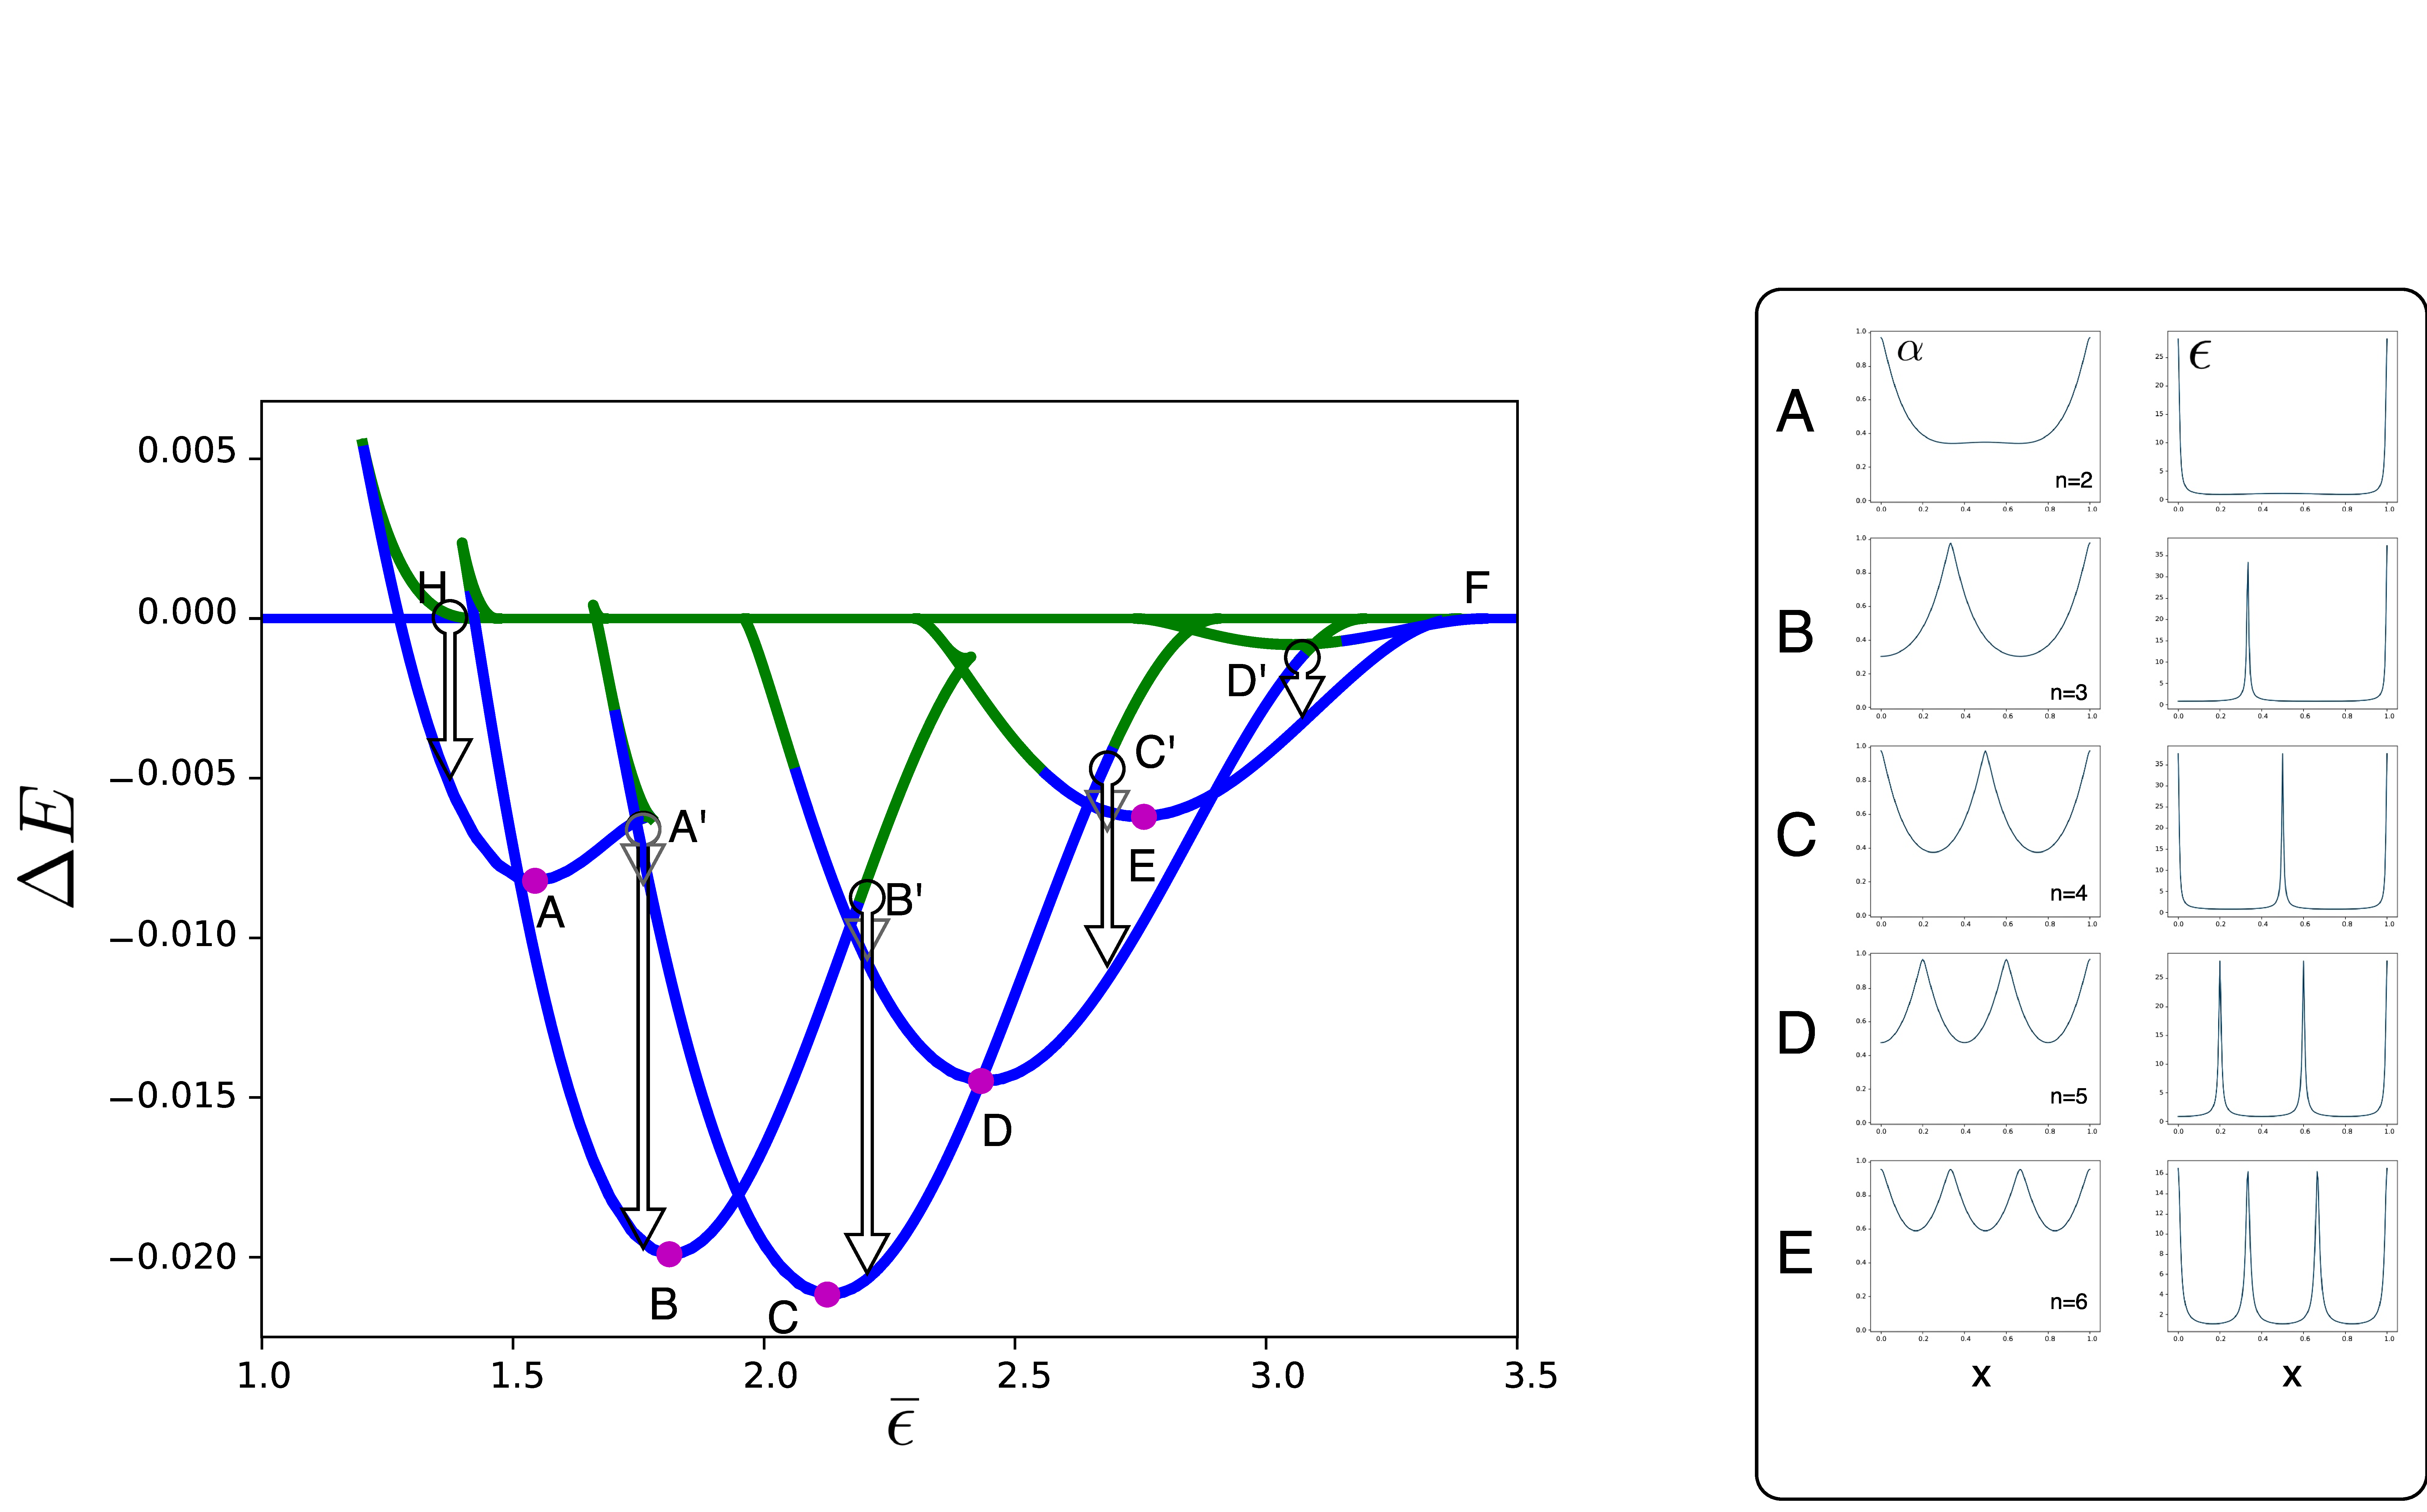
\includegraphics[scale=0.1]{./final_images/fig3.pdf}
\includegraphics[width=.8\textwidth]{../images/model_compliant_energy.pdf}
\includegraphics[width=.7\textwidth]{../images/model_compliant_fields.pdf}
\caption{
\todo[inline]{
    Add marker for $\ep_c, H$ in Fig (a)
    Add marker for $n=1, 2, ...$ in Fig (a)
    }
Equilibrium branches in the phase-field model of an elastic bar on non-rigid elastic foundation: (a) the energy difference $\Delta E$ between the affine and non-affine configurations. Stability of solutions is indicated by colors: blue denotes stability, while green indicates instability   via the numerical evaluation of the smallest eigenvalue of the stiffness matrix $\stiffmatcompl$; (b) the damage and strain profiles of the minimum energy configurations on each branch.}
    \label{fig:branches-compliant}
\end{figure}

We display the equilibrium branches that solve the nonlinear equations~\ref{auto1} in Fig. \ref{fig:branches-stiff}. These branches are represented in Figure~\ref{fig:branches-compliant} by plotting the energy difference $\Delta \Psi$, which represents the energy difference between the energy of the current non-affine solution and the energy of the homogeneous solution $\Psi_h(\bar{\epsilon})$ at the current value of the loading parameter $\bar\epsilon_t$. The stability of solutions is color-coded, XXXX and YYYY representing stable and unstable solutions, respectively.\comment{check palette and colour names} Stability is discerned through numerical evaluation of the smallest eigenvalue $\kappa$ of the stiffness matrix $\stiffmat$ defined in \eqref{eq:stifness1}. Eigenvalues represent the local curvatures of the energy functional, so the sign of the smallest  $\kappa$ determines the stability of the solution, with $\kappa > 0$ indicating stability and $\kappa < 0$ indicating instability.

Under the LEM protocol, the system explores the fundamental branch where the homogeneous solution is stable until $\bar\epsilon^c$, identified using linear stability analysis. SEE FIGURE XXX, DISPLAYING EVOLUTION XXXX. At the critical load $\bar\epsilon^c$  at point $H$, following the first instability, a branch switching transition occurs from the trivial branch with $n = 0$ to the nontrivial equilibrium branch with $n = 3$. The ensuing non-homogeneous configuration is linearly stable, as seen in Fig. \ref{fig:branches-stiff}. We depict the lowest energy configuration on this equilibrium branch in Fig.~\ref{fig:branches-stiff} at point A, consisting of two simultaneously nucleated localized cracks, one inside the domain and one on the boundary. 

When the loading parameter $\bar{\epsilon}$ is further increased, the equilibrium configuration with $n=3$ loses linear stability at point $A'$. In Fig. \ref{fig:branches-stiff} we represent state transitions by arrows, it can be observed that under the LEM protocol, the only available transition from point $A'$ is to the branch with $n=4$, which is locally stable within at the corresponding applied strain $\bar{\epsilon}$. The minimum energy configuration on the branch with $n=4$, depicted in Fig.~\ref{fig:branches-stiff} at point $B$, consists of two cracks: one inside the domain and two on the right and left boundaries.

Further increasing the load, the stability of the branch with $n=4$ is lost at point $B'$, a single available transition leads the system to the branch with $n=5$. While the branch with $n=6$ appears accessible due to its lower energy compared to the current state, it is unstable at the current value of $\bar\epsilon$. The lowest energy configurations on the branches with $n=5$ and $n=6$ are illustrated in Fig. \ref{fig:branches-stiff}(C-D). Increasing the load along the branch with $n=5$ which loses linear stability at point $C'$, a branch switching event occurs towards the branch with $n=7$, the corresponding minimum energy configuration on this branch is depicted in Fig.~\ref{fig:branches-stiff}(b). Finally, this branch reconnects to the homogeneous branch with $n=0$ at point $F$.

In the case of the compliant substrate model, the equilibrium branches that solve the nonlinear equations (Eq.~\ref{auto2}) are shown in Fig.~\ref{fig:branches-compliant}. 
We again plot the energy difference $\Delta \widetilde\Psi$ between the energy of the current solution and the energy of the homogeneous solution $f^0(\bar{\epsilon}, \alpha^0(\bar{\epsilon}))$ at the current value of the loading parameter $\bar\epsilon$. 
The stability of solutions is indicated by XXXXX and YYYYYY colors, representing stable and unstable solutions, respectively. Stability is now discerned through numerical evaluation of the smallest eigenvalue of the stiffness matrix $\stiffmatcompl$, defined in \eqref{eq:stifness2}.

According to the LEM protocol with a loading history starting in the unloaded and sound configuration, the initial transition from the trivial solution to the only available branch with $n=2$ occurs at $\epsilon_c^*$, marked as point H. As illustrated in Fig. \ref{fig:branches-compliant}(b), the damage and strain profiles of the lowest energy configuration at point A is characterised by two boundary cracks. As the loading increases, the system persists on the $n=2$ branch until point $A'$ which marks an instability. The system can now access two equilibrium branches: $n=3$ and $n=4$ shown in gray and black arrows. Fig. \ref{fig:branches-compliant}(b) shows the typical damage and strain profiles on these branches. Branches $n=3$ and $n=4$ show one bulk crack plus one boundary crack, and one bulk crack plus two boundary cracks, respectively. 

The choice of the subsequent branch transition at point $A'$ will dictate the ensuing crack growth. On branches with $n=3$ and $n=4$, at the instability points $B'$ and $C'$, the system will once again encounter two available equilibrium branches. From $n=3$ branch  at point $B'$, the system can transition to either the $n=4$ or $n=5$ branch. Opting for the $n=4$ branch, the subsequent branch selection occurs at point $C'$, offering branches with $n=6$ or $n=5$. Notably, the $n=5$ branch smoothly reconnects with the trivial solution at point $F$. However, the $n=6$ branch experiences another instability at point $D'$ before rejoining the trivial solution. 

The overall behavior of the compliant substrate model reveals, for the current choice of material parameters, additional complexity with more branch switching events and non-uniqueness of the overall response.\comment{asd}  In the stiff substrate model, the LEM strategy identifies a UNIQUE evolution path, while in the compliant substrate model the system can follow 8 different paths, GIVEN BY THE COMBINATION OF XXX DECISION-MAKING GAME. This additional complexity provides a good case to test numerical optimization methods, which we will discuss in the following.

\subsection{Equilibrium branch selection in overdamped viscous dynamic}
We consider now the equilibrium solutions reachable through the line-search based quasi-Newton algorithms such as  conjugate gradient or the BFGS optimization, which effectively  mimic the zero viscosity limit of overdamped viscous dynamics~\cite{SALMAN2012219}. Quasi-Newton methods serve as alternatives to Newton's method for locating roots or local extrema of functions. Particularly advantageous in scenarios where computing the Hessian at each iteration is impractical or computationally expensive, these methods circumvent the need for explicit computation \replaced[id=ALB]{of energy derivatives}{Hessian}. Instead, they rely on evaluating the function value and its gradient and updating the Hessian by analyzing successive gradient vectors.

Quasi-Newton methods are highly suitable for solving the phase-field equation of fracture, particularly when compared to standard Newton method-based monolithic solvers. Such solvers, which simultaneously  solve the equations for both damage and displacement variables, often falter when confronted with nonconvex energy functionals. For example, as demonstrated in \cite{Wick2017-bo}, the Newton method-based monolithic algorithm does not consistently handle brittle fracture scenarios involving abrupt crack propagation. Recently, quasi-Newton methods, particularly the BFGS variant, have been employed to effectively solve the system of coupled governing equations in a monolithic fashion within the phase-field method of fracture. These methods have demonstrated success in various engineering applications, as evidenced by \cite{Kristensen2020-zy,Wu2020-qk,Salman2021-mn,Liu2022-ix}.

In  this study, it is worth to note that our primary objective is not to provide a comprehensive assessment of quasi-Newton methods on a global scale. Instead, our focus lies in scrutinizing their behavior and performance specifically concerning equilibrium branch selections within our simplified framework, where all branches are readily identified. By narrowing our scope to this specific aspect, we aim to gain insights into the effectiveness and reliability of quasi-Newton methods in reaching the equilibrium states of our system.
\begin{figure}
    %\centering
% 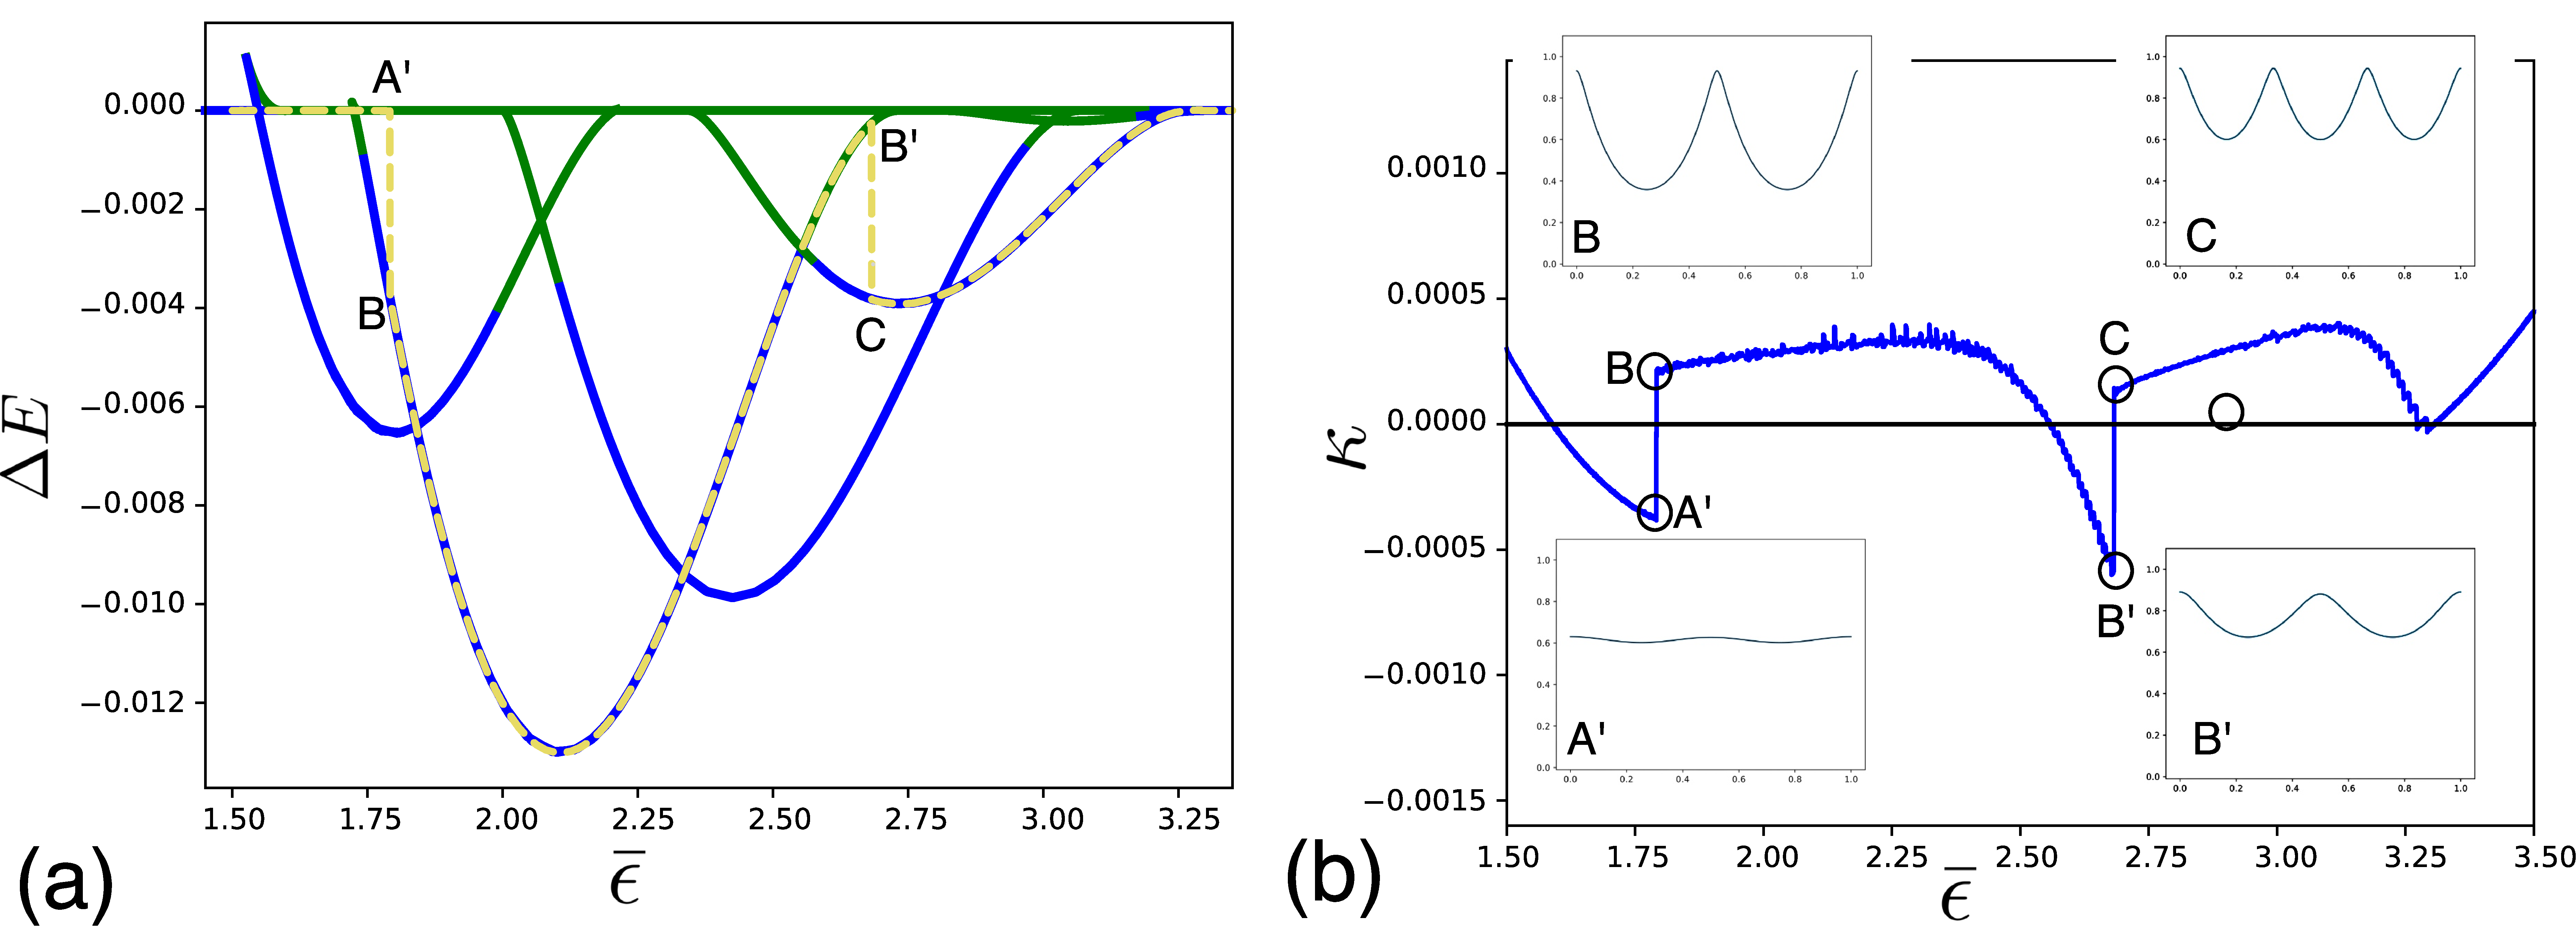
\includegraphics[scale=0.13]{./final_images/fig4.pdf}
\includegraphics[width=.7\textwidth]{../images/model_stiff_energy_kick.pdf}
\includegraphics[width=.4\textwidth]{../images/model_stiff_profiles.pdf}
    \caption{
% \todo[inline]{Add marker for $\ep_c, H$ in Fig (a) and (b)}
Quasi-static loading simulations with L-BFGS: (a) the energy difference $\Delta E$, between he quasi-Newton solutions (gray dashed line) and the homogeneous solutions are superimposed onto equilibrium branches (red); (b) smallest eigenvalue of the second variation  as a function of the loading parameter $\bar\epsilon$; inset show damage profiles.}
    \label{fig:tempo1}
\end{figure}

Recall that quasi-Newton algorithms only evaluate the function value and its gradient to reach equilibrium configurations. This implies that in our case, we need to evaluate integrals \eqref{modeld} and \eqref{model_elastic_substrate}, along with their first variations given by \eqref{firstvar1} and \eqref{firstvar}, in the first and second models, respectively. We   discretized the integrals \eqref{firstvar1} and \eqref{firstvar} to construct the residuals vectors using finite elements to obtain 
\begin{equation}
    {\bf R} =
    %  {\bf R}^1=
     \int_0^1 [(1-\alpha)^2u'\mathcal{N}'_i+\frac{1}{\lambda_2^2} (u-u_0) \mathcal{N}_i+\frac{1}{2}(u'^2 g'(\alpha)+h'(\alpha))\mathcal{N}_i+\lambda_1^2\alpha'\mathcal{N}'_i ]dx,\label{residual1}
\end{equation}
in the stiff model and 
\begin{equation}
    \widetilde{{\bf R}}= 
    % {\bf R}^2=
    \int_0^1 [(1-\alpha)^2u'\mathcal{N}'_i+\frac{1}{\lambda_2^2} (u-u_s) \mathcal{N}_i+\frac{1}{2}(u'^2 g'(\alpha)+h'(\alpha))\mathcal{N}_i+\lambda_1^2\alpha'\mathcal{N}'_i +r_su_s'\mathcal{N}_i]dx\label{residual2}.
\end{equation}
in the compliant substrate model. 

Among iterative methods for large-scale unconstrained optimization, particularly when dealing with possibly dense Hessian matrices,  quasi-Newton methods often emerge as preferable alternatives to the widely-used Newton-Raphson (NR) algorithm. The NR algorithm, conventionally utilized for solving linear equations to determine the correction $\Delta \mathbf{X}^{(k)}$ from the current estimate $\mathbf{X}^{(k)} = (\mathbf{u}^{(k)}, \boldsymbol{\alpha}^{(k)})$ at iteration $k$, is expressed in our context as:
\begin{equation}
K_{ij} \Delta X_j + R_i = 0,
\label{Eq:NR}
\end{equation}
where the discrete stiffness matrix $\mathbf{K}$ and bulk forces $\mathbf{R}$ are initialized with the initial guess $\mathbf{X}^{(k)}$. Subsequently, the guess is updated as $\mathbf{X}^{(k+1)} = \mathbf{X}^{(k)} + \Delta \mathbf{X}^{(k)}$ after solving Equation \eqref{Eq:NR} using LU factorization~\cite{Sanderson2016-ht}. It's evident that the NR algorithm fails if the discrete stiffness matrix $\mathbf{K}$ isn't invertible.

On the other hand, quasi-Newton methods are well-established (see standard textbooks, e.g., \cite{Nocedal1999-zr,Nocedal2006-qh}), and generate a sequence $\left\{\mathbf{X}^{(k)}\right\}$ according to the following scheme:
\begin{equation}
\mathbf{X}^{(k+1)} = \mathbf{X}^{(k)} + h^{(k)} \mathbf{p} ^{(k)}, \quad k=0,1,\ldots
\end{equation}
with
\begin{equation}
\mathbf{p}^{(k)}=-(\mathbf{B}^{(k)})^{-1}{\bf R},
\end{equation}
where $(\mathbf{B}^{(k)})^{-1}$ approximates the inverse of the Hessian matrix  $\mathbf{K}$ and $h^{(k)}$ represents a step length. Particularly, instead of computing $(\mathbf{B}^{(k)})^{-1}$  at each iteration $k$, these methods update $(\mathbf{B}^{(k)})^{-1}$ in a straightforward manner to obtain the new approximation $(\mathbf{B}^{(k+1)})^{-1}$  for the subsequent iteration. Additionally, rather than storing full dense $n \times n$ approximations, they only retain a few vectors of length $n$\comment{notation: $n$ already been used}, enabling implicit representation of the approximations. Moreover, the choice of the step length $h^{(k)}$ is carried out through a line search to minimize a function $f(h^{(k)}) = f(\mathbf{X}^{(k)} + h^{(k)} \mathbf{p}^{(k)})$ in order to find an acceptable step size $h^{(k)}$ such that $h^{(k)} \in \arg \min_{h} f$.

Among quasi-Newton schemes, the L-BFGS method is widely regarded as one of the most efficient and well-suited for large-scale problems due to its limited and user-controlled storage requirements. This method relies on constructing an approximation of the inverse Hessian matrix, leveraging curvature information solely from recent iterations. Note also that the update formula for the approximative in successive minimization steps depends on the adapted algorithm. These algorithms are extensively used in the literature, and we refer the reader to the references for a more detailed description~\cite{Matthies1979-gl,Xu2001-ax,Nocedal1999-zr,Nocedal2006-qh,Simone2012-tx,Lewis2013-eu,Curtis2015-wp}. However, quasi-Newton methods do present certain drawbacks, notably slow convergence for ill-conditioned problems, particularly when the eigenvalues of the Hessian matrix are widely dispersed~\cite{Simone2012-tx}.
\begin{figure}
    %\centering
    \includegraphics[width=.7\textwidth]{../images/model_compliant_energy_kick.pdf}
    \includegraphics[width=.4\textwidth]{../images/model_compliant_profiles.pdf}
    \caption{
        \todo[inline]{Add marker for $\ep_c, H$ in Fig (a) and (b),
        add $n=3, 4, ...$ in Fig (a),
        add $n=3, 4, ...$ in Fig (c)
        }
        Quasi-static loading simulations with L-BFGS: (a) the energy difference $\Delta E$, between the quasi-Newton solutions and the homogeneous solutions are superimposed onto equilibrium branches (red); (b) smallest eigenvalue of the second variation  as a function of the loading parameter $\bar\epsilon$; (c) damage profiles.}
    \label{fig:tempo2}
\end{figure}


In our numerical experiments, we employ the BFGS and L-BFGS solvers from the Python SciPy library~\cite{2020SciPy-NMeth} and the Alglib library~\cite{Bochkanov2013-lk}. These solvers utilize the residual vectors (see \ref{residual1} and \ref{residual2}) at each finite element node, alongside the values of integrals \eqref{modeld} and \eqref{model_elastic_substrate}.




\begin{figure}[htbp]
    \centering
    \includegraphics*[width=.45\textwidth]{../images/model_stiff_kick_profiles.png}
    \includegraphics*[width=.45\textwidth]{../images/model_compliant_kick_profiles.png}
    \caption{
        Profile of damage field showing the effect of the kick algorithm to transition from unstable to stable states. Branch switching events correspond to load values indicated by $\bar \epsilon_j$ with $j\in \mathbb N$ in Figure XXX, for the stiff substrate model (left column) and for the compliant substrate model (right column). %
        In the figures, the light (orange) line indicates the unstable damage field $\alpha^*$, the eigenvector associated to the smallest eigenvalue, $p$, is displayed in green highlighting its positive and negative values, the dashed line represents the perturbed damage field  $\alpha^*+p$ used as initial guess for the state transition, the solid black line displays the solution $\alpha$ returned by the quasi-Newton algorithm after convergence.}
    \label{fig:}
\end{figure}



% \begin{figure}
%     %\centering
% \includegraphics[width=\textwidth]{./final_images/fig6.pdf}
%     \caption{
% % \todo[inline]{Fix legend colours in (a)}
% Kick algorithm for the first model: (first column) the current unstable solution  for the damage field \added[id=ALB]{(blue)}, the \added[id=ALB]{eigenvector associated to the} smallest \replaced[id=ALB]{eigenvalue}{eigenvector} of this state \added[id=ALB]{(orange)}, and the perturbed damage field with this eigenvector \added[id=ALB]{(green)}; (second column)  the solution returned by the quasi-Newton algorithm wherein initial guess is taken to be the perturbed damage field.
%  }
    
%     \label{fig:kick}
% \end{figure}


% \begin{figure}
%     %\centering
% % \includegraphics[width=\textwidth]{./final_images/fig7.pdf}
%     \caption{Kick algorithm for the second model: (first column) the current unstable solution  for the damage field, the smallest eigenvector of this state, and the perturbed damage field with this eigenvector; (second column)  the solution returned by the quasi-Newton algorithm wherein initial guess is taken to be the perturbed damage field.
%  }
%  \label{fig:kick2}
% \end{figure}

%To summarize, we initially provide the algorithms with an initial guess for $\mathbf{X}^{(k)} = (\mathbf{u}^{(k)}, \alpha^{(k)})$ at a fixed value of the loading parameter $\bar\epsilon$. Additionally, we specify an initial guess for the Hessian matrix, denoted as $\mathbf{B}^{k} \in \mathbb{R}^{n \times n}$. This matrix can either be set as the identity matrix or the uncoupled stiffness matrix to ensure a symmetric and positive definite approximation. Subsequently, the quasi-Newton algorithm computes a search direction using  the analogue of the Newton equation $\mathbf{B}^{(k)} \mathbf{p}^{(k)}  = -\mathbf{R}^{(k)} $,where $\mathbf{p}^{(k)}$ denotes the search direction at stage $k$. Afterwards, it  performs a line search to minimize a function $f(h^{(k)}) = f(\mathbf{X}^{(k)} + h^{(k)} \mathbf{p}^{(k)})$ in order to find an acceptable step size $h^{(k)}$ such that $h^{(k)} \in \arg \min_{h} f$. The solution is then updated in the direction of $\mathbf{p}^{(k)}$ with the step size $h^{(k)}$. 


In Figure \ref{fig:tempo1}(a), we present the results of our numerical experiments, overlaying solutions obtained with the quasi-Newton algorithm onto equilibrium branches determined using the pseudo-arclength continuation method described in the previous section. Fig. \ref{fig:tempo1}(b) shows the smallest eigenvalue $\kappa$ whose positivity informs on the stability of the solution. All the branch switching events are delayed in the sense they do not take place when the smallest eigenvalue of the second variation vanishes but \added[id=ALB]{only beyond the load corresponding to the eigenvalue's sign transition.}. Notably, the expected first branch switching event—from the {homogeneous} solution to the branch with \(n=3\) as outlined in the LEM protocol—did not occur at point H as anticipated. During a monotonic loading, the system remains on the trivial branch, as shown in Fig. \ref{fig:branches-stiff}(a), until it transitions to the branch with \(n=4\) at a value of the load much higher than the critical loading parameter \(\bar{\epsilon}^c\). By monitoring the smallest eigenvalue of the second energy variation at the solution, we observe that indeed the solutions computed via the quasi-Newton solver are unstable beyond \(\bar{\epsilon}^c\), which is consistent with the linear stability results for the trivial branch. A closer inspection of the solution field reveals that the quasi-Newton solutions are not homogeneous but instead exhibit a small perturbation akin to the instability mode calculated analytically (i.e., the eigenvector associated with the smallest eigenvalue). For instance, the  quasi-Newton solution before the first branch switching event is shown in inset (A') in Fig. \ref{fig:tempo1}(b), where we see that \added[id=ALB]{the equilibrium damage shows a slight oscillation } reminiscent of the eigenmode \(\alpha_n(x) \sim \cos(n\pi x)\), \comment[id=ALB]{$\alpha_n(x) \sim c+ \cos(n\pi x)$ where $c$ is an arbitrary constant and} with \(n=3\) \textbf{what does it mean?}. The state transition captured by the quasi-Newton method is the one towards the  \(n=4\) branch, with one bulk crack and two boundary cracks, see inset (B) in Fig. \ref{fig:tempo1}(b). If the transition had taken place at \(\bar{\epsilon}^c\) as anticipated by our LEM strategy, the system would have reached a configuration with two bulk cracks and one boundary crack, as shown in Fig. \ref{fig:branches-stiff}(b) inset (A).

With continued loading, the damage increases and the system evolves along the \(n=4\) branch beyond the loading value at which stability is lost, as shown in Fig. \ref{fig:tempo1}(b). A dissipative branch switching event takes place from the current branch (\(n=4\)) at point \(B'\) to the branch with \(n=6\); see Fig. \ref{fig:tempo1}(b) and the inset C for the corresponding damage profile. The delay in bifurcation results in a branch selection event different from the one in our LEM protocol. The delays at bifurcation for the first and second branch switching events leads to a completely different evolutionary path compared to the LEM protocol until it finally reconnects with the homogeneous branch at point \(C'\).

After illustrating the numerical results for the stiff substrate model, we now transition to exploring the simulation results of with an compliant elastic background. The solutions of our numerical experiments obtained from the quasi-Newton algorithm (gray dashed line) are overlaid in Fig. \ref{fig:tempo2}(a) onto equilibrium branches, while their stability is depicted in Fig. \ref{fig:tempo2}(b). Notably, we observe a delay, albeit less pronounced compared to the stiff substrate model, for the bifurcation from the trivial branch which occurrs at a value  higher than the analytically determined critical load \(\bar{\epsilon}^c\). Interestingly, the quasi-Newton method switches to the branch with $n=2$, which exhibits lower energy compared to the branch with $n=3$. This occurs  despite the delay in bifurcation because the branch  $n=3$ remains accessible for the current value $\bar\epsilon$. It's worth noting that the LEM protocol also anticipated a first branch selection event leading to the branch with $n=2$ with two boundary cracks. 
We again observe that, \added[id=ALB]{even before the first branch-changing event}, the quasi-Newton solution \replaced[id=ALB]{is an homogeneous state perturbed by an oscillatory term of}{deviates from the trivial branch, and the damage profile has} the form \(\sim \cos(n\pi x)\), reminiscent of the eigenmode $\alpha_n$ \comment[id=ALB]{$\alpha_n(x) \sim c+ \cos(n\pi x)$ where $c$ is an arbitrary constant and} with \(n=2\) \textbf{what does it mean?}. 
% \added[id=ALB]{Remark: this may be due to the quasi-Newton computation which necessarily relies on an approximate positive-definite Hessian. EXPAND}
\added[id=ALB]{These perturbations of the equilibrium profiles are negligible from the global energetic standpoint, as it can be inferred in Figure~\ref{fig:tempo2}(a), by the superposition between the energy of the computed evolution and the exact total energy of the homogeneous solution.} 
As the load increases the system moves along the branch with $n=2$ until the stability transition at load XXX, indicated by point A'. Energy minimization brings the system to the branch $n=4$ although the branch with $n=3$ is also accessible and has lower energy. Figure~\ref{fig:tempo2}(c), displays the corresponding damage profiles before and after \added[id=ALB]{the branch} switching event  at points B' and C. The final \replaced[id=ALB]{transition}{event} before the reconnection to the homogeneous branch takes place at point C', which is also an unstable configuration. The transition brings the system to the branch $n=6$ as seen in Fig.~\ref{fig:tempo2}(b), the corresponding stable damage profile at point D is shown in Fig. \ref{fig:tempo2}(c). 

In summary, while the results of the quasi-Newton minimization simulations exhibit overall similarities in both models, the trajectory taken by the system in the second model more closely COMPARES with the LEM protocol outlined above. This alignment can be attributed to the specific energy landscape within the second model. HOWEVER, IN CASE OF INDETERMINACY SUCH AS WHEN MULTIPLE STABLE SOLUTIONS EXIST AT A LOSS OF STABILITY, WHERE SHOULD THE SYSTEM GO?

%: the states accessible to the system when the smallest eigenvalue vanishes remain unchanged compared to when the "delayed" branch switching occurs.

\subsection{Hybrid algorithm \added[id=ALB]{(kick) for branch switching}}
Our investigation reveals that the solutions generated by the quasi-Newton algorithms deviate from the prescribed LEM protocol outlined in the preceding sections. We observed a delayed bifurcation phenomenon and the persistence of unstable solutions, \replaced[id=ALB]{both affecting}{affect} branch selection events along the evolution.  This is indeed related to the fact that the energy landscape IS ALREADY flat when the determinant Hessian gets close to zero~\textbf{comment more}
\added[id=ALB]{
    Testing the energy expansion~\eqref{eqn:energy-expansion} 
    along a the direction of a bifurcation mode, that is setting $y-y_t=h w_n$, where $w_n:=(v_n, \alpha_n)(x)$ is the $n$-th eigenmode associated to the Hessian and $0<h\in \mathbb R$, we obtain that, for admissible states $y$ $\delta$-close to the equilibrium $y_t$ we can write the following lower bound}
$$
\Psi(y)-\Psi(y_t)\geq \frac{h^2}{2}\kappa \|w_0\|^2, \quad \forall y: \|y - y_t\| \leq \delta,
% \delta = O(\| y-y_t\|),
% +o(h^2\|w_n\|^2).
$$
\added[id=ALB]{where $\kappa$ indicates the smallest eigenvalue and $w_0$ the associated eigenmode. The first order term $\delta\Psi(y_t)(v_n, \alpha_n)$ vanishes identically owing to the fact that bifurcation modes are admissible fields for the equilibrium condition. 
When the smallest eigenvalue continuously approaches zero, the energy landscape morphs from being locally flat (at first order) and locally convex in all admissible directions including, in particular, the directions associated to the eigenmodes, to loosing local convexity in the one non-trivial direction associated to the eigenvalue that has changed sign. 
In the numerical practice, 
the convergence of quasi-Newton algorithms depends on the construction of an (approximate) strictly positive Hessian matrix.
As a consequence, such approximation systematically RULES OUT the ability to capture the change of sign (of the smallest eigenvalue) of the Hessian, that is its singularity, thus the onset of instability and the instability mode. 
This can justify the systematic (and algorithm-dependent) delay of the bifurcation events via the quasi-Newton solver, observed in figures~\ref{fig:tempo1} and~\ref{fig:tempo2}.}
To address this challenge, we introduce a hybrid approach \added[id=ALB]{that explicitly takes into account the singular mode of the Hessian}. In this method, we continuously monitor the smallest eigenvalue of the complete \replaced[id=ALB]{Hessian}{stiffness} matrix for the equilibrium solutions obtained from the quasi-Newton algorithm.\comment[id={ALB}]{why the notation capital bold $X$?}
When this eigenvalue significantly diminishes, indicating potential instability, we calculate the corresponding eigenvector, denoted as \(\mathbf{p}\). We then use this eigenvector to perturb the current solution $\mathbf{X^*}$. This perturbation sets the initial guess for the next minimization step in the quasi-Newton algorithm as $\mathbf{\tilde X}^{(0)} = \mathbf{X^*} + \eta \mathbf{p},
$ where \(\eta\) is the step size.\comment[id=ALB]{I removed the k indices}
\comment[id=ALB]{$\|\textbf{p}\|=1$}
% \comment[id=ALB]{Does $k$ refer to the quasi-Newton iteration number? I think it can be removed}
This step size can, in principle, be determined through a line-search algorithm by minimizing the one-dimensional energy slices along the energy descent mode given by the function 
$$f(\eta) = \Psi(\mathbf{X} + \eta \mathbf{p})
\label{eqn:energy-slice}$$
 to find an optimal value \(\eta\), such that $\eta \in \arg \min_{\eta} f$. One can Spectrum \(\eta = 1\)  \comment{is this still relevant?} (this choice is further discussed in the following) \added[id=ALB]{and run the quasi-Newton step to obtain a new critical point $\mathbf{\tilde X}$.}

The outcome of this hybrid algorithm ARE the three anticipated branch-switching events identified for the first model previously reported in Fig. \ref{fig:branches-stiff}. For each of these three cases, the snapshots of the damage fields, the associated \replaced[id=ALB]{instabilty mode}{ eigenvectors} \(\mathbf{p}\), \deleted[id=ALB]{and} the perturbed states \(\mathbf{\tilde X}^{(0)}\), and the converged solutions $\mathbf{\tilde X}$ are shown in Figs. \ref{fig:kick}(a,c,e).

When the quasi-Newton algorithm is initiated using the perturbed state \(\mathbf{\tilde X^{(0)}}\)
% \comment[id=ALB]{shouldn't the perturbed state read \(\mathbf{X}\)?} 
as the initial guess, \replaced[id=ALB]{a state transition}{ bifurcation} occurs which leads the system into a qualitatively different state, cf. the final  converged solutions returned from the quasi-Newton minimization are shown in Figs. \ref{fig:kick}(b,d,f). For the stiff substrate model, the \replaced[id=ALB]{instability mode}{ smallest eigenmode} which corresponds to the bifurcation from the trivial branch has the form \(\cos(n\pi x)\) with \(n=3\), as identified through the linear stability analysis (see Fig. \ref{fig:kick}(a)). 
The perturbad quasi-Newton minimization returns a state with two boundary cracks and one interior crack, as shown in Fig. \ref{fig:kick}(b), which corresponds to the solution found using the arc-length continuation algorithm on the branch with \(n=3\) (see Fig. \ref{fig:branches-stiff}(b), inset A).  The hybrid algorithm is also successful in capturing the next two anticipated branch   switching events: from the  branch with \(n=3\)  to the branch  with \(n=4\) (see Fig. \ref{fig:kick}(d)) and  from branch with \(n=4\)  to the branch  with \(n=5\) (see Fig. \ref{fig:kick}(f)). The hybrid algorithm is able to capture the unique path dictated by the LEM protocol shown in Fig. \ref{fig:branches-stiff}.   

LET'S focus on the compliant substrate model. In this case, according to the LEM protocol, the path through which the system may evolve under quasi-static loading is not unique due to the multiplicity of (stable) solutions at critical loads.
%  i.e., external strain at which the stability of a branch is lost,  and, will be determined by the minimization algorithm.
Note that this is not the case for the first model wherein there is a single equilibrium branch accessible to the system for all given critical loads.\comment[id=ALB]{double check}
Despite the fact that quasi-Newton algorithm was able to reproduce one of the possible paths predicted by the LEM protocol for the compliant substrate model, the \replaced[id=ALB]{the branch switching events}{ optimal path may be different due to the delays  in} \added[id=ALB]{are delayed with respect to the} anticipated bifurcations. 


The system's response under the hybrid algorithm is depicted in Fig. \ref{fig:kick2}. The first column displays the perturbed damage profiles, while the second column shows the outcomes of the energy minimization process starting from  this perturbed state. Initially, a stable state with two nucleated boundary cracks (branch \( n=2 \)) is achieved following the destabilization of the trivial branch, as illustrated in Fig. \ref{fig:kick2}(b). Subsequently, an interior crack nucleates in the middle of the system (branch \( n=4 \)), as shown in Fig. \ref{fig:kick2}(d). The third event involves a transition from branch \( n=3 \) to branch \( n=5 \). The final event depicted in Fig. \ref{fig:kick2} is the transition to branch \( n=6 \). The last event before reconnecting to the trivial branch is the transition from branch \( n=6 \) to branch \( n=7 \), the only  branch available to the system at this load. To summarize, the branches selected by the hybrid algorithm follow the sequence 
\( 0 \rightarrow 2 \rightarrow 3 \rightarrow 5 \rightarrow 6 \rightarrow 7 \rightarrow 0 \), 
which differs from the sequence 
\( 0 \rightarrow 2 \rightarrow 3 \rightarrow 4 \rightarrow 6 \rightarrow 7 \rightarrow 0 \) 
followed by the quasi-Newton algorithm.

Finally, we will discuss the determination of the step-size \( \eta \) used to obtain the perturbed state as the initial guess for the quasi-Newton algorithm.
\replaced[id=ALB]{Our numerical findings suggest that equilibria close to the Hessian degeneracy (i.e. with small but positive eigenvalues) are robust in the sense that they are insensitive to perturbations. This is highlighed by the fact that running the quasi-Newton solver on a perturbed state close to the Hessian sign transition yields, after convergence, the same equilibrium state prior to perturbation.
On the other hand, when the smallest eigenvalue of the system's Hessian is small and negative, the
small value of the step size \( \eta \) obtained by minimisation of \eqref{eqn:energy-slice} is not sufficient for the quasi-Newton algorithm to effectively escape the flat region of the energy landscape. 
}{ However, in our case, the smallest eigenvalue of the system's Hessian is slightly less than zero, resulting in a very small \( \eta \) that prevents the quasi-Newton algorithm from escaping the flat region of the energy landscape.}

To escape this region, one can design an iterative algorithm that repeatedly performs line searches in the current unstable direction until stability is found, iteratively flowing along the escape path. However, for the current problem, it was sufficient to take the step-size \( \eta=1 \) to escape the unstable critical states, even though this choice is suboptimal \replaced[id=ALB]{with respect to}{increases the function} \( f(\eta) \). 
% Indeed, the essential feature of the quasi-Newton algorithm is the positive definiteness of the approximate Hessian, independent of the function's curvature (positive or negative). 
The quasi-Newton solver starting from the perturbed state seeks a direction that will always be a descent direction. Therefore, a perturbed state obtained by taking a large step-size moves the system away from the flat region, allowing the quasi-Newton algorithm to find the next lower energy branch. It remains to be seen if this choice will work in other models or a more elaborated algorithm has to be implemented, as suggested above, which will be the subject of future work.
\begin{figure}
    %\centering
    \includegraphics[width=.7\textwidth]{../images/model_stiff_energy_kick_algo.pdf} \\
    \includegraphics[width=.7\textwidth]{../images/model_compliant_energy_kick_algo.pdf}
    \caption{
        % Quasi-static loading simulations with L-BFGS: (a) the energy difference $\Delta E$, between the quasi-Newton solutions and the homogeneous solutions are superimposed onto equilibrium branches (red); (b) smallest eigenvalue of the second variation  as a function of the loading parameter $\bar\epsilon$; (c) damage profiles.
        }
    \label{fig:tempo2}
\end{figure}


\subsection{\added[id=ALB]{Irreversibility and numerics} }
\added[id=ALB]{
To conclude this contribution and highlight the role of the irreversibility constraint on the global definition of space of perturbations, 
we qualitatively discuss the full stability problem~\eqref{eq:variational_stability} in our simplified one-dimensional setting, for an initially undamaged thin film on a stiff substrate undergoing a homogeneous evolution, and provide an illustrative numerical computation. 
As a pointwise constraint, irreversibility restricts branch switching events in such a way that, e.g., the transition between branches with $n=3$ to $n=4$  is not allowed (cf. profiles in the Figure~\ref{fig:kick1} of the transition (b)$\mapsto$ (d)) because it requires a local decrease of the damage field. 
On the flip side, irreversibility also acts as a global constraint on the perturbation space rendering the analysis more involed because of the strong nonlinearity induced.
}

% The former is determined by the smallest eigenvalue of the operator $H(y)$, which is a non-linear operator that depends on the current damage state, whereas the latter is determined by the eigenvalue problem in the vector space.
\added[id=ALB]{
We perform a one-dimensional test using the same parameters as in the experiment~\ref{sec:rigid} for the rigid substrate model, plotting in Figure~\ref{fig:irreversibility}-top the profiles of the fields at the loading step corresponding with point H in Figure~\ref{fig:branches-stiff}.
More precisely, we plot the homogeneous damage field $\alpha_h$ and represent the profiles of the damage eigenfunctions associated to the minimal eigenvalue both for the second order bifurcation~\eqref{eq:variational_inequality} (left panel) and stability problem~\eqref{eq:variational_stability} (right panel).
The bifurcation profiles coincide with the eigenmodes $n=4$ alredy found, cf.~Figure~\ref{fig:}
}
\added[id=ALB]{
Note that the profiles of the instability modes do not reduce to a truncation (i.e. a projection on the cone $K^+_0$) of the bifurcation modes, and this is due to the necessary regularity of the solutions requiring continuity of first derivatives. 
In Figure~\ref{fig:irreversibility}-bottom, we plot the spectra of the Hessian operator for the bifurcation problem (with blue circles and red crosses) as well as the smallest eigenvalue in the irreversible stability problem (with losanges). 
Note that the bifurcation spectrum is singular at $t=0$. This follows the fact that, in this model, the damage criterion is attained as soon as $t=0$, thus the space of state perturbations changes suddenly from $H^1_t((0,1)) \times \emptyset$ at $t=0$ to the full space $V_0$ for $t>0$ which includes all (sufficiently smooth) damage perturbations. Conversely, the set of admissible damage perturbations for the stability problem changes from the empty at $t=0$ set to the solid cone of smooth positive functions $\{\beta\in H^1((0,1)):\beta \geq 0\}$ only beyond the bifurcation load, that is for $t>t_b>0$.
In the inset, we zoom on the infimum of the spectra which shows the transition from the uniqueness of the homogeneous branch (with a strictly positive Hessian in the vector space) to the existence, for $t \geq t_b$, of a multiplicity of negative eigenvalues corresponding to equilibrium curves passing through the current homogeneous state, each of which associated to a bifurcation mode.
Despite the occurrence of negative eigenvalues for the bifurcation problem, the eigenvalues of the stability problem are all positive, indicating the sufficient condition for stability of the computed evolution.
}
% the numerical solution indicates that there exists a sequence of positive eigenvalues for the full stability problem, indicating the sufficient condition for stability of the computed evolution.
% Note that eigenvalues of the stability problem are only computed for $t\geq t_b$, as the uniqueness of the evolution branch ensures stability for $t<t_b$.
% }
% Put in perspective with previous JMPS artcle.

% An image of the eigenmode which was inadmissible, meaning nucleation does not occur at the critical load of the reversible model. After showing that, we can further discuss the localization of the first crack formation. 
% Alternatively, we could mention that the irreversible case is more complex and that branch selection requires separate work using the tools in your JMPS.


\begin{figure}[htbp]
    \centering
    % \includegraphics*[width=.7\textwidth]{../images/spectra-7f4361886184f3c6791fe16bf4f4b3f2.pdf}
    % \includegraphics*[width=.7\textwidth]{../images/spectra-zoom-7f4361886184f3c6791fe16bf4f4b3f2.pdf}
    \caption{Spectrum of the Hessian $\Psi''(y_t)$ at equilibrium for the rate bifurcation problem (circles) and irreversible stability problem (losanges), rescaled with respect to the minimum eigenvalue of the purely elastic phase at $\bar \epsilon = 0$. At load $\bar \epsilon_b$, the bifurcation problem is singular and the trajectory in phase space looses its uniqueness. 
    Corresponding to the gray shaded area, the detail of the inf-spectra are shown in the right figure. The transition from the uniqueness of the homogeneous branch to the existence of a multiplicity of equilibrium curves passing through the current homogeneous state is shown by the change of sign of the inf-eigenvalue and the existence of multiple negative eigenvalues. For $\bar \epsilon \geq \bar \epsilon_b$ multiple equilibrium paths cross the current state. The inf-eigenvalue of the stability problem in the restricted space $K^+_0$ is positive, indicating a sufficient condition for stability of the computed evolution. The tolerance for the numerical computation of the inf-eigenvalue is $10^{-6}$.}
    \label{fig:irreversibility}
\end{figure}


\begin{figure}[htbp]
    \centering
    \includegraphics*[width=.95\textwidth]{../images/profiles-bif-stab-7f4361886184f3c6791fe16bf4f4b3f2.pdf}
    \label{fig:irreversibility}
    \caption{Profiles of the damage field at the bifurcation load $\bar \epsilon_b$ and of the inf-eigenvector for the bifurcation (left) and stability (right) problems. The bifurcation profile coincides with the eigenmode $n=...$ alredy found, cf.~\eqref{}, its associated eigenvalue is $\kappa = -9\cdot 10^{-4}$. The inf-eigenvector of the stability problem is a smooth non-negative function corresponding to $\kappa=2\cdot 10^{-2}$.}
\end{figure}

------



\begin{figure}[htbp]
    \centering
    \includegraphics*[width=.7\textwidth]{../images/irreversibility_inf_eig.png}
    \caption{The right solver should'nt give you a crack.
    SECOND ORDER ANALYSIS OF THE HOMOGENEOUS SOLUTIONS. UNIQUENESS, LOSS OF UNIQUENESS, STABILITY. NOTICE THAT THE STABILITY-OBSERVABLE (MARKER) IS \emph{DISCONTINUOUS}.
    % (THE MARKET SHOUDN'T GIVE YOU A CRACK. THE MARKET DOESN'T GIVE A FUCK.) 
    }
    \label{fig:shouldnt}
\end{figure}

We have compared the performance of the algorithm proposed in this paper with aN continuation method, DEFINED AS FOLLOWS (EXPERIMENTAL). 


\begin{figure}[htbp]
    \centering
    \includegraphics*[width=.7\textwidth]{../images/VSA*.png}
    \caption{STABILITY (DIS)CONTNIUATION ALGORITHM, THE OUTER LOOP IDENTIFIES ONE TIMESTEP, THE ITERATIVE K-PERTURBATIONS ARE PERFORMED AT FIXED LOAD.}
    \label{fig:shouldnt}
\end{figure}

FROM NUMERICAL EXPERIENCE, SOLUTIONS TO XXX (The former) exhibit SENSITIVITY TO numerical bifurcation artifacts, while SOLUTIONS TO [DEF], consistently maintain the THE OBSERVABILITY OF homogeneous solution. (SINGULAR PROBLEM)

In Figure~\ref{fig:shouldnt}, we EXHIBIT THE CONSEQUENCES OF a NUMERICAL EFFECTS that emphasiSes the role of the irreversibility constraint in our STABILITY-DRIVEN optimiSation approach. THE NUMERICAL SETTING IS THAT OF THE FIRST the PART OF THE paper, where OSCILLATIONS AROUND the homogeneous solution WERE INVESTIGATED AS THE RESULTS OF A BIFURCATION ANALYSIS. Specifically, DESPITE slight numerical fluctuations MANIFESTING AS wavy (SINUSOIDAL) patternS, AND DESPITE THAT THE INF-EIG-CONE EVOLVES DISCONTINUOUSLY, the homogeneous solution IS INDEED stable AND SHOULD BE OBSERVED.

IN FACT, Applying a standard Newton-Raphson monolithic solver to this  wavy-PERTURBED TEST solutionS, the expected nucleation of cracks does not occur, WHICH IS IN AGREEMENT TO THE STATEMENT IN [DEF]. This lack of crack nucleation contrasts with our NUMERICAL RESULTS OBTAINED using the conjugate gradient method combined with an active-set irreversibility approach. To the best of our knowledge, this discrepancy is aN INTERESTING numerical artifact rather than a physical phenomenon.